\documentclass[twocolumn]{article}

\usepackage[utf8]{inputenc}
\usepackage{mathtools}
\usepackage{amssymb}
\usepackage{amsmath}
\usepackage{hyperref}

\usepackage[authoryear]{natbib}
\bibliographystyle{plainnat}

\usepackage{svg}

\usepackage{etoolbox}

\makeatletter

\pretocmd{\NAT@citex}{%
  \let\NAT@hyper@\NAT@hyper@citex
  \def\NAT@postnote{#2}%
  \setcounter{NAT@total@cites}{0}%
  \setcounter{NAT@count@cites}{0}%
  \forcsvlist{\stepcounter{NAT@total@cites}\@gobble}{#3}}{}{}
\newcounter{NAT@total@cites}
\newcounter{NAT@count@cites}
\def\NAT@postnote{}

% include postnote and \citet closing bracket in hyperlink
\def\NAT@hyper@citex#1{%
  \stepcounter{NAT@count@cites}%
  \hyper@natlinkstart{\@citeb\@extra@b@citeb}#1%
  \ifnumequal{\value{NAT@count@cites}}{\value{NAT@total@cites}}
    {\ifNAT@swa\else\if*\NAT@postnote*\else%
     \NAT@cmt\NAT@postnote\global\def\NAT@postnote{}\fi\fi}{}%
  \ifNAT@swa\else\if\relax\NAT@date\relax
  \else\NAT@@close\global\let\NAT@nm\@empty\fi\fi% avoid compact citations
  \hyper@natlinkend}
\renewcommand\hyper@natlinkbreak[2]{#1}

% avoid extraneous postnotes, closing brackets
\patchcmd{\NAT@citex}
  {\ifNAT@swa\else\if*#2*\else\NAT@cmt#2\fi
   \if\relax\NAT@date\relax\else\NAT@@close\fi\fi}{}{}{}
\patchcmd{\NAT@citex}
  {\if\relax\NAT@date\relax\NAT@def@citea\else\NAT@def@citea@close\fi}
  {\if\relax\NAT@date\relax\NAT@def@citea\else\NAT@def@citea@space\fi}{}{}
\hypersetup{
    bookmarks=true,
    unicode=false,
    pdftoolbar=true,
    pdfmenubar=true,
    pdffitwindow=false,
    pdfstartview={FitH},
    pdftitle={My title},
    pdfauthor={Author},
    pdfsubject={Subject},
    pdfcreator={Creator},
    pdfproducer={Producer},
    pdfkeywords={keyword1} {key2} {key3},
    pdfnewwindow=true,
    colorlinks=false,
    linkcolor=red,
    citecolor=green,
    filecolor=magenta,
    urlcolor=cyan
}

\title{Recognizing Printed Melodies using Object Detection and a Convolution Neural Network}
\author{Onur Kocahan and Friedrich Hartmann}

\begin{document}
 
\maketitle
\section{Introduction}
The goal of Optical Music Recognition (OMR) is to reproduce a sequence of document-written musical notation by a machine. Since the language of musical notation contains hundreds of symbols, this problems becomes really complex. \\
Our aim is to to treat only a fragment of the musical notation language, namely the fragment of American and Europe folk music. It has a huge restriction on the alphabet, since it does not contain chords, for example, and is more appropriate of our use case. Because we want to apply OMR to an application that photocopies a tune of a song-book and transforms it later to an audio file. This can be further used to learn how to sing this tune.  \\
Available OMR Datasets such as DeepScores \citep{DeepScores} contains around 30 000 000 sheets of written music with close to a hundred millions of small objects. This would really blow up our project. That's why we generate our own Dataset. \\
We further follow the general framework to OMR that contains according to \citet{state_of_the_art} the following steps. 
\begin{enumerate}
 \item image pre-processing
 \item recognition of the musical symbols;
 \item reconstruction of the musical information in order to build a logical description of musical notation; and
 \item construction of a musical notation model to be represented as a symbolic description of the musical sheet.
\end{enumerate}
The most challenging task in this framework is point 2. An common approach to that is to use Neural Networks. A baseline for that is given by \citet{Baseline}. The authors applied Faster R-CNN, RetinaNet and U-Net on various datasets. The performance on DeepScores, which is not hand-written and therefore easier be trained, is not promising as the mean average precisions of the intersection over union ratios are 19.6\%, 9.8\%, and 24.8\%, respectively. \\
An other approach by \citet{GitHub_OMR} is more promising, but has really good results around 95\% only for a selection where the bounding boxes have at least an intersection over union ratio of 0.50. \\
That's why we invent a new approach on the object detection that is not based on a neural net.\\ We further apply a Convolutional Nueronal Network to classify the outputs of our objects detection mechanism which are then be used to generate an audio file. \\
Implementation details can be read up in our GitHub project \url{https://github.com/lutacluny/Sheet-Music-Recognition}.


\section{Musical Notation Background}
This section is about giving the reader a short summary of musical notation.\\
There exists various styles of writing music, but we focus only on the modern staff notation which is characterized by a staff line. \\
The position of the note head determines its name. It can be on the line, between two lines and above or under the staff using ledger lines. Therefore, limiting the ledger lines to one upper and one lower, a line can hold 13 different notes. \\
The value of a note is specified by its shape and defines its duration which is given relatively to the beat. That means that the note value \textit{quarter} has the length of a quarter beat. \\
A visualization of the explanations above is given in \hyperref[musical_notation]{Figure 1}. 
Other musical symbols do not depend on its vertical position at the line. 


\begin{figure}
 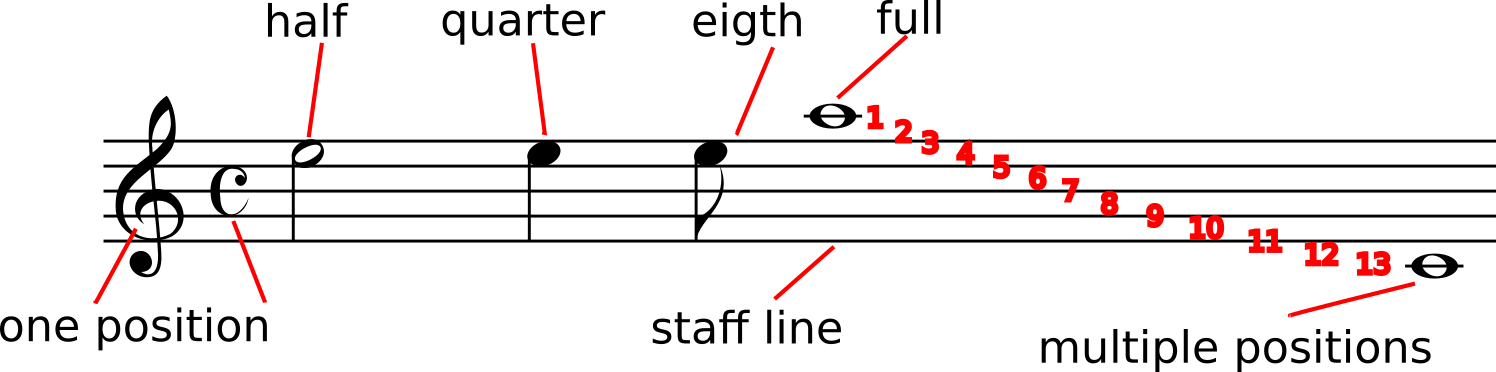
\includegraphics[width=\linewidth]{notation.png}
 \caption{Musical notation simplified}
 \label{musical_notation}
\end{figure}

\section{Training Data Sampling}
We build a highly flexible framework to generate a database that contains image files which can be used to train a Neuronal Net. It is build of musical symbols extracted as vector graphics by the help of the tool abc2mps \citet{abc2mps}. \\
As one generated image file per musical symbol is not sufficient for training, we introduced several parameters for data augmentation. These are output dimension, scaling, rotation, horizontal shift, vertical shift and the respective number of outputs in the ranges defined by these parameters. It is for example possible to get 5 output files with respect to the scaling in the range $80\%$ to $120\%$. \\
Our database supports at the moment up to 107 different musical symbols. Therefore, the number of training examples is $107 \cdot N$, where $N$ is the number of augmented files per symbol. 

\section{Object Detection}
In this section we describe our approach on the object detection. As the input is a single image file, the general task is to split this image into several images, such that each of the resulting images contains one and only one musical symbol which can be recognized by a machine. The first step is to transform the image from RBG into black and white. \\
Our idea is further based on the observation that tunes of American and European folk music, written in the modern staff notation, contain recurrent patterns which is illustrated by \hyperref[object_detection]{Figure 2}. \\
As it can be observed, each line, colored black, has the same height and width. Furthermore, the distance between two lines remains the same. That gives the possibility to identify first the most upper line and then calculate the position of the other lines. This can be achieved by representing the image as a matrix and identifying a column, that contains only staff lines. Because such a column has a unique pattern on the distances between the lines, which can be easily calculated on the matrix. The red colored line illustrates this fact in \hyperref[object_detection]{Figure 2}. \\
After segmentation of the lines we split each line into symbols or groups of symbols, until each of the resulting segments contains one and only one symbol. To accomplish this, we take advantage of the fact that a column of the respective matrix representation associated with a line, has a significantly bigger amount of black pixels. The reference value of a column without a note is calculated identifying a column that matches the orange line in  \hyperref[object_detection]{Figure 2}. This is performed the same way as for the red marked column. 

\begin{figure}
 \includesvg[width=\linewidth]{object_detection.svg}
 \caption{Abstracting a tune} 
 \label{object_detection}
\end{figure}

The success of this procedures depends on photo quality. It is mandatory that the staff lines are parallel to the edges of the photocopy. But in practice, this not really an issue, since most cameras have a grid implemented. \\
Furthermore, there are two hyper-parameters that needs to be chosen appropriated. Like we explained before, what matters is the amount of black pixels per column. So, there needs to be a thresh hold that separates columns containing musical symbols from those containing only staff lines. This is given as $\epsilon_{black}$ in per cent. The second one ,$\delta$, is the separate width, given as a fraction of the images width. Only columns marked as containing a note, for which its distance exceeds the separate width, are split. \\
It turned out that $\epsilon_{black} = 60\% $ and $\delta = 1/120$ in the first run and $\epsilon_{black} = 140\%$ and $\delta = 1/10$ in the second shows desirable results. Our test images are split into 543 different images. It holds further that each new image contains one and only one musical symbol. The quality is shown in \hyperref[quality]{Figure 3}.

\begin{figure}
\begin{tabular}{l|l l l l}
 percentage of symbol  \\
 contained in the image  & $ < 50 $ & $ < 90 $ & $ < 100$ & $100$ \\
 \hline \\
 & 1 & 11 & 65 & 487 
\end{tabular}
\caption{For example, it can be observed that on 54 images $10 \%$ of the symbol is not visible anymore.}
\label{quality}
\end{figure}


It has to be finally admitted that choosing the right values for $\epsilon_{black}$ and $\delta$ is challenging. Finding a promising strategy on that, which performs good apart form our test suite, is not part of this project.  





\section{Image Classification}
foo

\section{Post Processing}
The final step is to transform the output labels into an audio file. This is performed by first converting the output labels into a format that can be processed by PySynth \cite{pysynth} which is the tool that generates the audio file. 


\newpage 


\bibliography{ref.bib}  

\end{document}

